\section{Task 6 --- Launching a Man-In-The-Middle Attack with
a Compromised CA}
%
\begin{lstlisting}[caption=A command generating a Certificate Signing
    Request for the fake Facebook website, label={lst:csr_script_fake_facebook}]
    openssl req -newkey rsa:2048 -sha256 \
    -keyout facebook.key -out facebook.csr \
    -subj "/CN=www.facebook.com/O=Meta Inc./C=US" \
    -passout pass:dees
\end{lstlisting}

\begin{lstlisting}[caption=A command generating a Certificate for the
    fake Facebook website, label={lst:crt_script_fake_facebook}]
    openssl ca -config demoCA_openssl.cnf \
    -policy policy_anything -md sha256 -days 365 \
    -in facebook.csr -out facebook.crt -batch \
    -cert ca.crt -keyfile ca.key
\end{lstlisting}

\begin{lstlisting}[caption={\fontfamily{qcr}\selectfont VirtualHost} entry for
    fake {\fontfamily{qcr}\selectfont www.facebook.com},
    label={lst:virtual_host_entry}]
    <VirtualHost *:443>
        DocumentRoot /var/www/bank32
        ServerName www.facebook.com
        DirectoryIndex index.html
        SSLEngine On
        SSLCertificateFile /volumes/facebook.crt
        SSLCertificateKeyFile /volumes/facebook.key
    </VirtualHost>
\end{lstlisting}

\begin{figure}
    \centering
    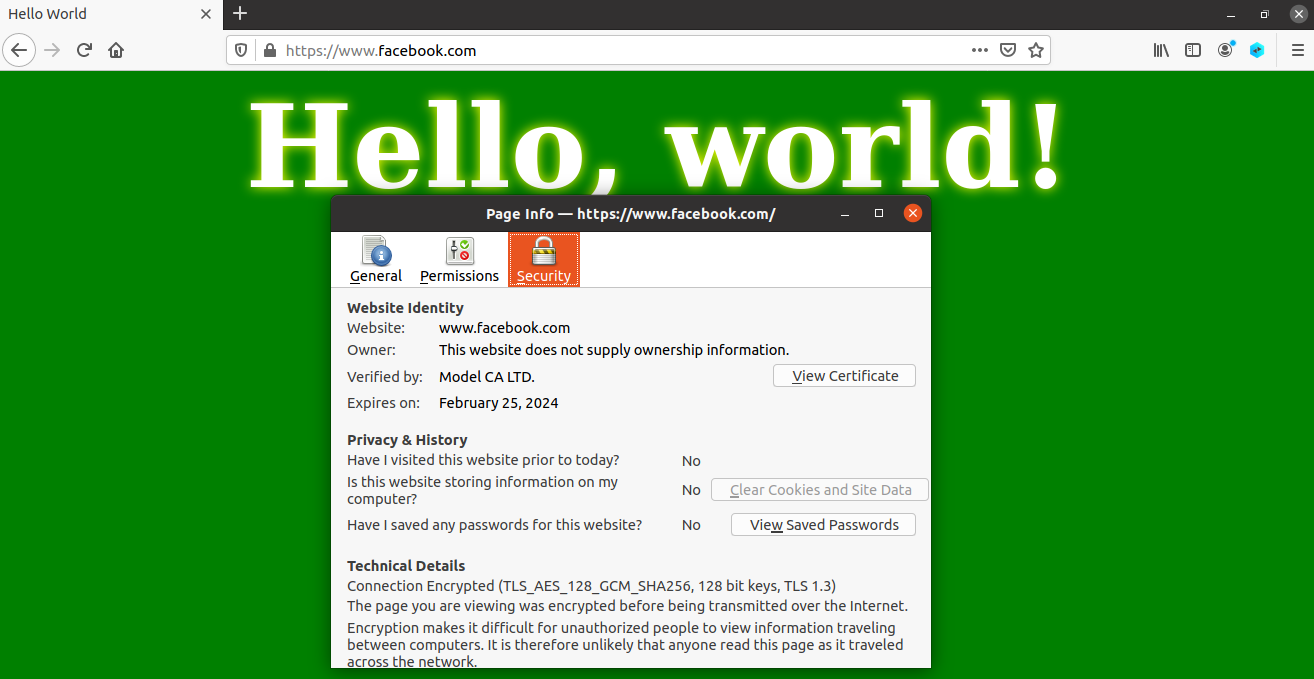
\includegraphics[height=\textheight,width=\textwidth,keepaspectratio]
    {figures/fake_facebook.png}
    \caption{Fake {\fontfamily{qcr}\selectfont www.facebook.com}
    can be accessed without any errors or warnings}
    \label{fig:fake_facebook}
\end{figure}

In this work, we selected the popular
social network Facebook ({\fontfamily{qcr}\selectfont www.facebook.com}) as the
target website. 
As mentioned in the SEED's instruction, the attacker can generate any arbitrary
certificate using the stolen CA's private key. We demonstrate that attack by generating
a certificate that is issued by our root CA for our fake Facebook website. Firstly,
we produced a CSR (see \autoref{lst:csr_script_fake_facebook}). Then we signed using
the compromised CA's private key (see \autoref{lst:crt_script_fake_facebook}). After
we got the certificate stored in {\fontfamily{qcr}\selectfont facebook.crt} and the
private key binding to that certificate {\fontfamily{qcr}\selectfont facebook.key},
we copied those two files into the shared folder {\fontfamily{qcr}\selectfont volumes}.
Next, we added the {\fontfamily{qcr}\selectfont VirtualHost} entry in {\fontfamily{qcr}\selectfont
bank32\_apache\_ssl.conf} (see \autoref{lst:virtual_host_entry}). Consequently, our
fake Facebook website can be visited without any errors or warnings raised by Firefox.
Addtionally, we can see that HTTPS secure connection was shown while we were visiting
the website (see \autoref{fig:fake_facebook}). In conclusion, this experiment shows that
an attacker can do a MITM attack with a compromised root CA.
